\documentclass[a4paper]{article}
\usepackage[utf8]{inputenc}
\usepackage[russian]{babel}
\usepackage[T2]{fontenc}
\usepackage[warn]{mathtext}
\usepackage{graphicx}
\usepackage{amsmath}
\usepackage{floatflt}
\usepackage[left=20mm, top=20mm, right=20mm, bottom=20mm, footskip=10mm]{geometry}


\graphicspath{ {images/} }
\usepackage{multicol}
\setlength{\columnsep}{2cm}


\begin{document}

\begin{titlepage}
	\centering
	\vspace{5cm}
	{\scshape\LARGE Московский физико-технический институт \par}
	\vspace{4cm}
	{\scshape\Large Лабораторная работа \par}
	\vspace{1cm}
	{\huge\bfseries Интерферометр Жамена \par}
	\vspace{1cm}
	\vfill
\begin{flushright}
	{\large выполнила студентка 653 группы ФФКЭ}\par
	\vspace{0.3cm}
	{\LARGE Карпова Татьяна}
\end{flushright}
	

	\vfill

% Bottom of the page
	Долгопрудный, 2018 г.
\end{titlepage}

\section{Цель работы}
Знакомство с техникой интерференционных измерений показателей преломления газов с помощью интерферометра Жамена

\section{В работе используются:}
\begin{itemize}
    \item интерферометр Жамена
    \item газовая кювета
    \item осветитель
    \item зрительная труда
    \item сильфон
    \item баллон с углекислым газом
    \item манометр
    \item краны
    \item светофильтр
\end{itemize}

\section{Теоретические положения}
В одну из камер вводится исследуемый газ, а вторая заполнена воздухом при атмосферном давлении. При этом разность хода, вызванная $\triangle$, вызванная разностью показателей преломления газов $\delta n$, приводит к сдвигу интерференционных полос:
\begin{equation}
    \triangle = \delta n l => \delta n = m \frac{\lambda}{l},
\end{equation}
так как сдвиг на одну полосу соответствует дополнительной разности хода $\triangle = \lambda$ \par
Показатель преломления исследуемого газа определяется путем сравнения с воздухом при атмосферном давлении:
\begin{equation}
    n = n_0 + \frac{\triangle}{l}
\end{equation}

\section{Схема установки}

Принципиальная схема интерферометра Жамена показана на рис. 1

    \begin{figure}[h]
    \centering
    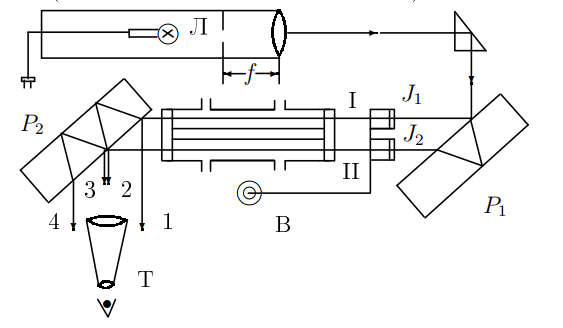
\includegraphics[width=10cm]{fig1.PNG}
    \caption{Интерферометр Жамена}
    \label{fig:vac}
\end{figure}

\section{Ход работы}

\begin{enumerate}
    \item Ознакомимся с принципом работы установки. Проведём юстировку и калибровку прибора. Для калибровки наденем на окуляр красный светофильтр и снимем зависимость показаний микрометрической шкалы компенсатора Жамена от порядкового номера интерференционного максимума. Результаты измерений занесём в таблицу 1 и графически представим на рис. 2
    
        \begin{table}[h]
    \centering
    \begin{center}
    \caption{Калибровка компенсатора}
    \end{center}
    \vspace{0.1cm}
    \label{tab:my_label}
    \begin{tabular}{ |p{1cm}||p{0.5cm}|p{0.5cm}|p{0.5cm}|p{0.5cm}|p{0.5cm}|p{0.5cm}|p{0.5cm}|p{0.5cm}| p{0.5cm}|p{0.5cm}|p{0.5cm}|p{0.5cm}|p{0.5cm}|p{0.5cm}|p{0.5cm}|p{0.5cm}| p{0.5cm}|}
 \hline
$m$ & -8 & -7 & -6 & -5 & -4 & -3 & -2 & -1 & 0 & 1 & 2 & 3 & 4 & 5 & 6 & 7 & 8\\
 \hline
 $z, \mu m$ & -10 & -4 & 3.5 & 10 & 16 & 22 & 29 & 35 & 42 & 48.5 & 54.5 & 62 & 68 & 75 & 81 & 88 & 94.5\\

 \hline
 
\end{tabular}
\end{table}

    \begin{figure}[h]
    \centering
    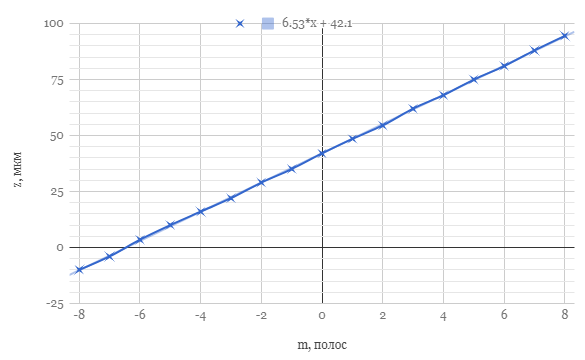
\includegraphics[width=15cm]{graph2.PNG}
    \caption{График калибровки компенсатора}
    \label{fig:vac}
\end{figure}

При этом длина кюветы $l = 10 $см, а длина волны, пропускаемая светофильтром $\lambda = 650 $нм.

\item По формуле (2) перейдём от делений компенсатора к величине $\delta n$
\begin{equation}
    \delta n = m\frac{\lambda}{l},
\end{equation}
при этом по рис. 2 $\triangle m = \frac{\triangle z}{\tan \varphi}$, где $\tan \varphi = 6.53$ - угол наклона калибровочного графика. Тогда окончательно

\begin{equation}
    \delta n = \frac{\triangle z}{\tan \varphi} \frac{\lambda}{l} = 10^{-6} \triangle z
\end{equation}

\item Изменяя давление с помощью сильфона, снимем зависимость показаний компенсатора $z$ от перепада давлений $\triangle P$. Результаты занесём в таблицу 2.

    \begin{table}[h]
    \centering
    \begin{center}
    \caption{Зависимость показаний микрометра от давления}
    \end{center}
    \vspace{0.1cm}
    \label{tab:my_label}
    \begin{tabular}{ |p{1.5cm}||p{0.5cm}|p{0.5cm}|p{0.5cm}|p{0.5cm}|p{0.5cm}|p{0.5cm}|p{0.5cm}|p{0.5cm}| p{0.5cm}|p{0.5cm}|p{0.5cm}|p{0.5cm}|p{0.5cm}|p{0.5cm}|p{0.6cm}|}
 \hline
$P, $ кПа & 7 & 6 & 5 & 4 & 3 & 2 & 1 & 0 & -1 & -2 & -3 & -4 & -5 & -6 & -6.5\\
 \hline
 $z, \mu m$ & 69 & 65.5 & 63 & 59.5 & 57 & 53.5 & 51 & 47 & 45.5 & 42 & 39 & 36 & 33 & 29.5 & 28\\

 \hline
 
\end{tabular}
\end{table}

    \begin{figure}[h]
    \centering
    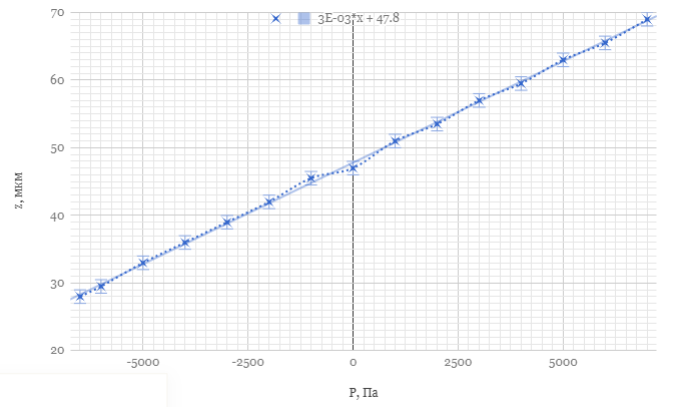
\includegraphics[width=15cm]{graph1.PNG}
    \caption{Зависимость показаний микрометра от давления}
    \label{fig:vac}
\end{figure}

Угол наклона графика $\tan \theta = 3*10^{-3}$

\item Определим среднюю поляризуемость молекулы воздуха:

\begin{equation}
\delta n = \frac{2 \pi \alpha}{kT} \triangle P
\end{equation}

\begin{equation}
\alpha = \frac{\delta n kT}{2 \pi \triangle P} = \frac{\triangle z \lambda}{\tan \varphi l} \frac{kT}{2 \pi \triangle P} =\frac{\tan \theta}{\tan \phi} \frac{\lambda kT}{2 \pi l \triangle P} = 193*10^{-32}
\end{equation}

Табличное значение составляет $\alpha = 172 * 10^{-32}$

Погрешность измерения определим по стандартной формуле (умножение величин), погрешность измерения углов наклона определим методом наименьших квадратов.
\begin{equation}
\sigma_{\alpha} = \alpha\sqrt{(\frac{\sigma_{\tan \theta}}{\tan \theta})^2 + (\frac{\sigma_{\tan \varphi}}{\tan \varphi})^2 + (\frac{\sigma_{T}}{T})^2 + (\frac{\sigma_{l}}{l})^2 + (\frac{\sigma_{\triangle P}}{\triangle P})^2} = 10 \hspace{1cm} \varepsilon = 5.3\%
\end{equation}

\item Определим показатель преломления воздуха по формуле
\begin{equation}
    n = 1 + 2\pi\alpha \frac{P}{kT} = 1.000303
\end{equation}

Для $T = 295$ K и $P = 102$ кПа
\begin{equation}
    n = 1 + \frac{(n_0 - 1)T_0 P}{T P_0} = 1.000283
\end{equation}

Аналогично п. 4, погрешность определения показателя преломления составляет 
\begin{equation}
    \sigma_n = 0.000018 \hspace{1cm} \varepsilon = 6 \%
\end{equation}

В пределах погрешность теоретический и экспериментальный результаты совпадают.

\item По результатам измерений оценим радиус молекулы азота, приняв молекулу за металлический шарик в однородном электрическом поле. Из задачи о проводниковом шаре в электрическом шаре, дипольный момент его будет равен $p = 3V E_0$, но в то же время $p = \alpha E$ из определения
Получили, что 
\begin{equation}
    \alpha = 3 V => r \sim \alpha^{1/3} \sim 10^{-10} m
\end{equation}

Реальный радиус молекулы азота также составляет порядка $10^{-10}$ м, наша оценка верна

\item Во вторую кювету запустим углекислый газ. Сразу после этого набежит разность хода, которая компенсируется поднятием компенсатора на 190 мкм.

Так как $n_2 - n_1 = \delta n$, а $\delta n$ была определена по формуле через калибровочный график, $\delta n = \triangle z \frac{\lambda}{l \tan \varphi} = 0.995 \triangle z$

Поэтому 
\begin{equation}
    n_{CO2} = n + 0.995\triangle z = 1.000303 + 0.000189 = 1.000492 \pm 0.000032
\end{equation} 
Погрешности определены аналогично предыдущим пунктам, и в их пределах результаты практически совпадают: при данных Т и Р $n_{CO2} = 1.000420$

\end{enumerate}

\section{Вывод}

В ходе работы был изучен принцип работы интерферометра Жамена, а также экспериментально определены следующие различные величины:
\begin{itemize}
    \item поляризуемость молекулы воздуха:
    $$\alpha_{exp} = 193*10^{-32} \pm 10 \hspace{2cm} \alpha_{th} = 172*10^{-32}$$
    \item показатель преломления воздуха при $T = 295$ К и $P = 102$ кПа:
    $$n_{exp} = 1.000303 \pm 0.000018 \hspace{2cm} n_{th} = 1.000283$$
    \item оценен радиус молекулы азота:
    $$r \sim 10^{-10} m$$
    \item показатель преломления углекислого газа при $T = 295$ К и $P = 102$ кПа:
    $$n_{exp} = 1.000492 \pm 0.000032 \hspace n_{th} = 1.000420$$
\end{itemize}

Хотя и существуют более точные интерферометры, интерферометр Жамена хорошо подходит для определения этих параметров.

\end{document}
